\begin{figure}%
    \centering
    \subfloat[]{{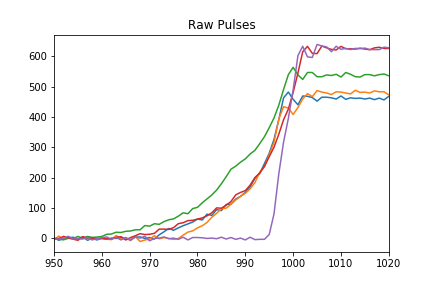
\includegraphics[width=7cm]{./figures/tenevents_rawdata.pdf} }}%
    \quad
    \subfloat[]{{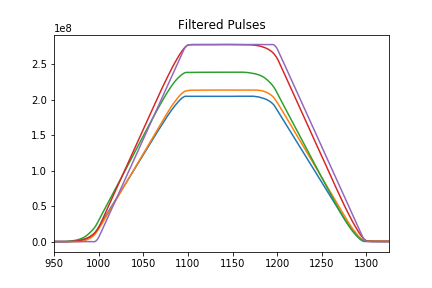
\includegraphics[width=7cm]{./figures/tenevents_filtered.pdf} }}%
    \caption{In figure (a) 5 sample events are shown. In figure (b) are the five signals after the application of a trapezoidanl filter with a gap time and peaking time of 1 $\mu$s. Note that the time interval on both plots in in ADC samples, which are each 10 ns apart in time.}%
    \label{fig:signals}%
\end{figure}

Five signals were chosen from the ${}^{137}{Cs}$ data set. The raw signals are plotted in \ref{fig:signals}, after a baseline correction. The resultant signals after usage of the trapezoidal filter with a gap time and peaking time of 1 $\mu$s are also plotted. The correlation between amplitudes can be seen. The signal in purple exhibits ideal behavior, with sharp edges and a flat top. This signal corresponds to the unfiltered signal with the fastest rise-time. All of the charge is collected quickly and the unfiltered signal more closely resembles an ideal step function. The red signal is of the same amplitude but has a longer rise time. As expected, the resultant trapezoid is less ideal, showing more curved corners and more variation in amplitude in the flat top region. These effects can lead to degraded energy resolution.

If the gap time of a filter is too small, ballistic deficit can be seen. This happens when filter rise time and gap time are not large enough to allow full charge collection. Making the gap time longer negates this effect. However, making the gap time too long can give the filter worse noise performance. 

In this implementation the effects of ballistic deficit on energy resolution can be seen. For small gap times, the peak position is shifted down in energy. Also, the peak is broader and tends to have low-energy tailing. Some of this is likely due to ballistic deficit. For gap times greater than a certain amount ($\approx$)250 ns, no significant variation in energy resolution with increasing gap time was observed. This value corresponds roughly to the largest transit time for charge carriers expected in a small coaxial HPGe detector (on the order of hundreds of ns \cite{Knoll} ), as expected.

A plot of resolution as a function of gap time is shown in \ref{gap}.

\begin{figure}[]
\begin{centering}
\includegraphics[width=0.8\textwidth]{gap_optimization_co.pdf}
\caption{Energy resolution as a function of gap time for the 1173 keV peak in ${}^{60}$Co. The peaking time was kept fixed at 500 ns. The errors shown only account for fitting errors.}
\label{gap}
\end{centering}
\end{figure}
\vspace{5mm}

\begin{figure}[]
\begin{centering}
\includegraphics[width=0.8\textwidth]{peak_optimization_co.pdf}
\caption{Energy resolution as a function of peaking time for the 1173 keV peak in ${}^{60}$Co. The gap time was kept fixed at 450 ns. The errors shown only account for fitting errors.}
\label{peak}
\end{centering}
\end{figure}
\vspace{5mm}

\begin{figure}[]
\begin{centering}
\includegraphics[width=0.8\textwidth]{fwhm_vs_energy.pdf}
\caption{Energy resolution as a function of gamma energy is plotted. Error bars account for fitting errors. These error bars are smaller than the markers and thus not visible.}
\label{peak}
\end{centering}
\end{figure}
\vspace{5mm}

If the gap time of a filter is too small, ballistic deficit can be seen. This happens when filter rise time and gap time are not large enough to allow full charge collection. Making the gap time longer negates this effect. However, making the gap time too long can give the filter worse noise performance. 
If the gap time of a filter is too small, ballistic deficit can be seen. This happens when filter rise time and gap time are not large enough to allow full charge collection. Making the gap time longer negates this effect. However, making the gap time too long can give the filter worse noise performance. 